%%%%%%%%%%%%%%%%%%%%%%%%%%%%%%%%%%%%%%%%%%%
%%%%%%%%%%%%%%%%%%%%%%%%%%%%%%%%%%%%%%%%%%%
%%%%%%%%%%%%%%% CHAPTER 04 %%%%%%%%%%%%%%%%


\section{Arquitetura da automação industrial}

\frame{
\frametitle{Arquitetura da automação industrial}
\begin{block}{Introdução}
\begin{itemize}
    \item Dentro da automação industrial, nós temos diversos tipos de \textbf{sensores de campo} para fazer a medição e detecção de determinado variável de processo. Esses sensores de campo enviam as informações de processo utilizando \textbf{protocolos industriais ou padrões de comunicação}.
    \item Tudo isso é concentrado em um sistema responsável por \textbf{controlar e atuar nos elementos finais de controle}. Todo controle tem como intuito manter a produção dentro do que é determinado, ou seja, manter a qualidade e segurança do processo.
\end{itemize}
\end{block}
}

\frame{
\frametitle{Pirâmide da automação industrial}
\begin{block}{Introdução}
\begin{itemize}
    \item Para uma fácil compreensão de toda essa estrutura de comunicação e instrumentos de medição, nós temos a \textbf{pirâmide da automação industrial}.
    \item Basicamente, esta pirâmide nos dá um \textbf{entendimento mais simplificado de de todos os níveis de comunicação em uma solução completa de automação industrial}. Além disso, temos todos os equipamentos, instrumentos de medição e controladores que fazem parte da pirâmide da automação industrial.
\end{itemize}
\end{block}
}

\frame{
\frametitle{Pirâmide da automação industrial}
\centerline{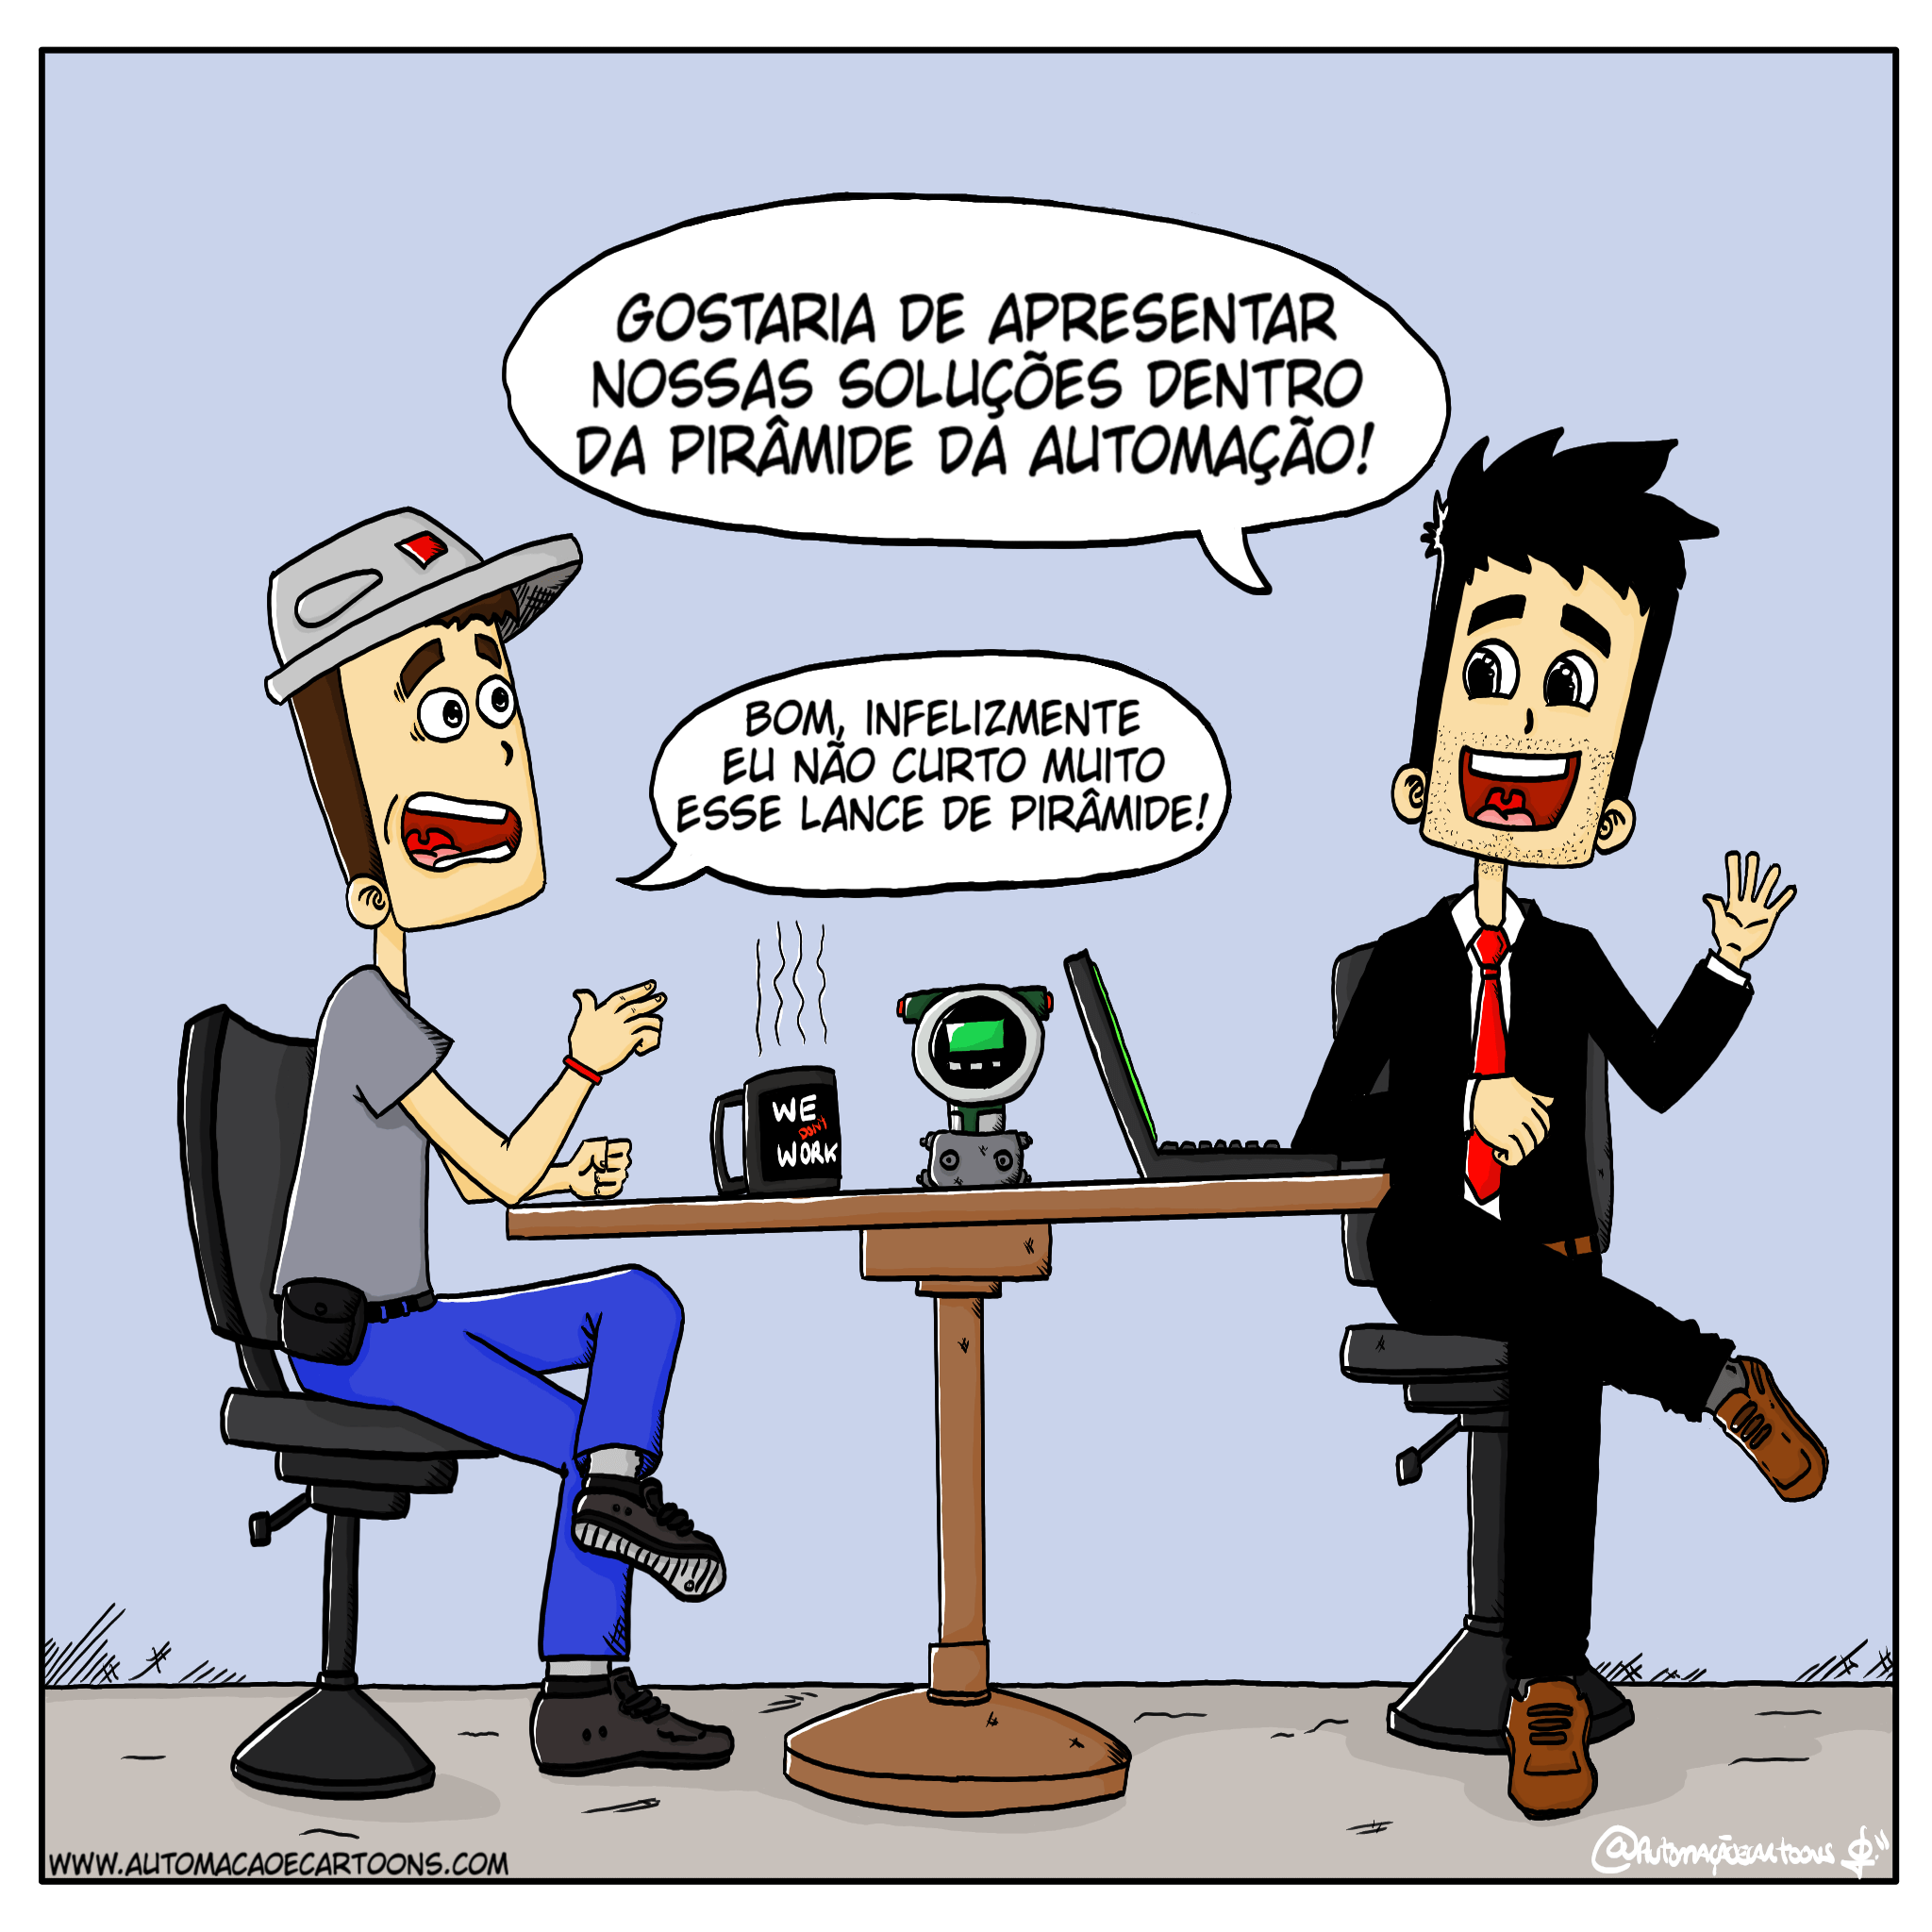
\includegraphics[width=0.65\linewidth]{Figuras/Ch04/fig4.png}}
}

\frame{
\frametitle{Pirâmide da automação industrial}
\begin{block}{Definição}
\begin{itemize}
    \item Primeiramente, a pirâmide da automação industrial é dividida em \textbf{5 níveis}, que conectados, utilizam  diferentes tipos de protocolos de comunicação.
\end{itemize}
\end{block}
\centerline{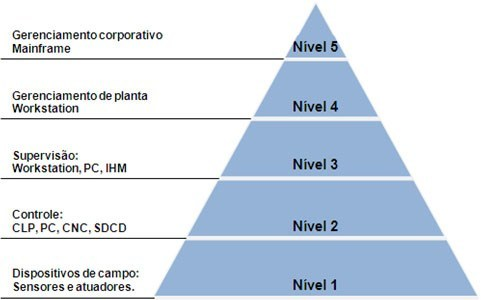
\includegraphics[width=0.7\linewidth]{Figuras/Ch04/fig1.jpg}}
}

\frame{
\frametitle{Nível 1 - aquisição de dados e controle manual}
\begin{block}{Sensores e atuadores}
\begin{itemize}
    \item Este nível é a \textbf{base na pirâmide da automação industrial}. Antes de fazer o controle do processo é necessário fazer as \textbf{medições de processo}.
    \item Os instrumentos de campo ou dispositivos de campo podem ser \textbf{simples}, não exigindo muita configuração e ainda, fornecendo uma saída de comunicação sem diagnósticos ou configurações sofisticadas.
    \item Hoje em dia, temos os instrumentos inteligentes ou \textbf{smart devices}. Tais instrumentos de medição tem uma configuração sofisticada e uma maior flexibilidade de aplicação. Além disso, você tem diagnósticos e a possibilidade de integração utilizando protocolos digitais.
    \item Outro item importante no nível 1 são os \textbf{atuadores ou elementos finais de controle}. Assim que a informação de processo é enviada para os controladores, eles devem atuar nos elementos finais de controle mantendo o \textit{setpoint} da malha de controle.
\end{itemize}
\end{block}
}

\frame{
\frametitle{Nível 1 - aquisição de dados e controle manual}
\begin{block}{Padrão de comunicação 4 - 20 mA}
\begin{itemize}
    \item Toda informação no campo é \textbf{enviada utilizando protocolos de comunicação digitais ou analógicos}. A comunicação \textbf{4-20 mA} é mais comum mesmo nos dias atuais, pois é \textbf{simples e bem robusta}. Todavia, temos outros protocolos que reduzem custos de implementação, além de dar acesso a diagnóstico e acesso remoto dos equipamentos, como PROFIBUS DP/PA, FOUNDATION Fieldbus, HART, WirelessHART, Ethernet-IP, PROFINET, entre outros.
    \item Equipamentos com saída de sinal na forma 4 a 20 mA, por terem sua saídas em corrente, tendem a ser \textbf{mais imunes a ruído elétrico e interferências externas}. Geralmente, entradas de equipamentos preparados para receberem sinais do tipo 4 a 20 mA possuem uma impedância de entrada baixa, menor de $\SI{500}{\ohm}$, sendo $\SI{250}{\ohm}$ um valor bastante comum, que ajuda a atenuar o ruído, resultando num sinal mais “limpo”.
\end{itemize}
\end{block}
}

\frame{
\frametitle{Nível 1 - aquisição de dados e controle manual}
\begin{block}{Padrão de comunicação 4 - 20 mA}
\begin{itemize}
    \item Mas por que $\SI{250}{\ohm}$ é um valor comum para uma saída 4 a 20mA? Pois, neste caso, quando tivermos 4 mA, teremos 1 V na entrada de sinal ($\SI{250}{\ohm}$ x 0,004 A = 1 V) e em 20 mA teremos 5V ($\SI{250}{\ohm}$ x 0,020 A = 5 V). Assim, \textbf{este sinal poderá ser aplicado diretamente em uma entrada de microcontrolador, que possui, na maioria das vezes, uma entrada 0 a 5 V}.
    \item Outra vantagem deste tipo de saída é que se a conexão entre a entrada e a saída do sinal se romper, \textbf{será percebido a falta de corrente no circuito}, o que resulta 0 mA na entrada de sinal. Como em condições normais a corrente nunca é 0 mA (fica sempre entre 4 e 20 mA), \textbf{a falta de corrente indicaria falha na conexão ou falha em algum dos equipamentos que estão interligados}.
\end{itemize}
\end{block}
}

\frame{
\frametitle{Nível 1 - aquisição de dados e controle manual}
\begin{block}{Padrão de comunicação 4 - 20 mA}
\begin{itemize}
    \item Mais um ponto a favor da saída 4 a 20 mA é referente a um \textbf{melhor resultado em ligações à distância}. Como a saída é em corrente, não há perda de sinal no caminho.
    \item Poderíamos citar como \textbf{desvantagem} deste padrão de sinal o fato de termos certa \textbf{limitação da quantidade de equipamentos a serem conectados em uma única saída}. Ao contrário dos sinais de saída em tensão, não podemos colocar entradas em paralelo, pois o sinal em corrente se dividiria entres as diferentes entradas causando um grande erro de leitura.
\end{itemize}
\end{block}
}

\frame{
\frametitle{Nível 1 - aquisição de dados e controle manual}
\begin{block}{Chão de fábrica}
\begin{itemize}
    \item Este nível também é conhecido como \textbf{chão de fábrica}, e o principal objetivo é o de \textbf{transferir dados entre o processo e o sistema de controle}.
\end{itemize}
\end{block}
\centerline{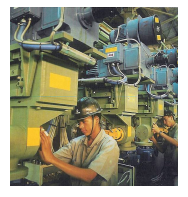
\includegraphics[width=0.4\linewidth]{Figuras/Ch04/fig2.PNG}}
}

\frame{
\frametitle{Nível 2 - controle individual}
\begin{block}{CLP, SDCD...}
\begin{itemize}
    \item Aqui encontramos o \textbf{“cérebro da planta”}. Todo os controles de processos são feitos neste nível utilizando equipamentos sofisticados para realizar as estratégias de controle.
    \item O \textbf{CLP} (Controlador lógico programável) está localizado neste nível, além do \textbf{SDCD} (Sistema Digital de Controle Distribuído), entre outros.
\end{itemize}
\end{block}
}

\frame{
\frametitle{Nível 3 - controle de célula, supervisão e otimização do processo}
\begin{block}{Sistemas supervisórios}
\begin{itemize}
    \item Como o nome já diz, neste nível temos soluções para realizar a \textbf{supervisão do processo industrial}.
    \item Existem diversas formas de supervisionar o que está acontecendo no campo, como também fazer o \textbf{controle remoto}. 
    \item Uma outra função realizada nesta camada é a de \textbf{banco de dados}, onde é feito o armazenamento das informações de processo, para uma análise futura do comportamento da malha de controle.
\end{itemize}
\end{block}
}

\frame{
\frametitle{Nível 3 - controle de célula, supervisão e otimização do processo}
\begin{block}{Sistemas supervisórios}
\begin{itemize}
    \item Soluções como \textbf{SCADA}, \textbf{IHM} (Interface Homem-Máquina) e Workstation estão localizadas na camada nível 3. Toda conexão entre o sistema de controle e o sistema de supervisão é feita utilizando conversores ou protocolos aberta na grande maioria, como OPC, OPC UA, Modbus, etc.
\end{itemize}
\end{block}
\centerline{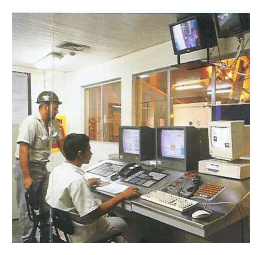
\includegraphics[width=0.4\linewidth]{Figuras/Ch04/fig3.PNG}}
}

\frame{
\frametitle{Nível 4 - gerenciamento da planta industrial}
\begin{block}{Controle fabril total, produção e programação}
\begin{itemize}
    \item Na produção, é necessário ter um controle e gestão das matéria prima, quantidade que deve ser produzida e demais recursos. O nível 4 é responsável pelo \textbf{planejamento, controle e logística dos suprimentos}.
    \item Para realizar a gestão dos suprimentos, ferramentas como MES e PIMS utilizam como base o \textbf{banco de dados e relatórios gerados no nível 3}.
    \item A troca de informação neste nível é feita baseada em \textbf{Ethernet}, além de utilizar banco de dados para armazenamento das informações e gerar relatórios.
\end{itemize}
\end{block}
}

\frame{
\frametitle{Nível 5 - gerenciamento corporativo}
\begin{block}{Planejamento estratégico}
\begin{itemize}
    \item O nível da informação neste nível é \textbf{corporativo}, focado na área de vendas e gestão do recursos. Essas informações tem como intuito gerar \textbf{melhores resultados financeiros para a empresa}.
    \item Neste nível encontram-se softwares para gestão de venda, gestão financeira e BI (Business Intelligence) para ajudar na \textbf{tomada de decisões} que afetam a empresa como um todo.
\end{itemize}
\end{block}
}

\frame{
\frametitle{Exercícios}
\begin{block}{}
01. Considerando a pirâmide de automação industrial, a aquisição de dados da planta industrial e o controle de automatização são realizados, respectivamente, em quais níveis?

\vspace{0.5cm}

02. Em uma pirâmide de níveis de automação, tem-se da base para o topo o nível chão de fábrica, o nível de campo, o nível de células e, no topo, o nível de administração.
Sabe-se que cada nível de comunicação tem sua finalidade específica. Nesse contexto, as entradas e saídas de sinal dos sensores e atuadores encontram-se em qual nível?

\vspace{0.5cm}

03. Por que se utiliza a entrada analógica do CLP numa escala de 4 a 20 mA, e não 0 a 20 mA?
\end{block}
}

\section*{Referências}
\frame{
\frametitle{Referências e Exercícios Complementares}
\begin{itemize}
\item NATALE, F. Automação Industrial. 10 ed. São Paulo: Érica, 2013.
\end{itemize}
%\centering{\alert{Página 546 - \textbf{Capítulo 6}}} \\
%\centering{\alert{Lista de exercícios 01}}
}